\documentclass[runningheads]{llncs}
\usepackage{graphicx}
\usepackage[text={150mm,220mm},centering,nohead]{geometry}
\pagestyle{empty}

\usepackage{graphicx}	%加入图片包


%\documentclass[GBK]{ctexart}
\usepackage{listings}	%代码段要导入的包
\usepackage{xcolor}
\lstset{
    %backgroundcolor=\color{red!50!green!50!blue!50},%代码块背景色为浅灰色
    rulesepcolor= \color{gray}, %代码块边框颜色
    breaklines=true,  %代码过长则换行
    numbers=left, %行号在左侧显示
    numberstyle= \small,%行号字体
    %keywordstyle= \color{red},%关键字颜色
    commentstyle=\color{gray}, %注释颜色
    frame=shadowbox%用方框框住代码块
    }



\begin{document}
\title{\large{CSCI927 Service-Oriented Software Engineering (Project Report)}}
\author{}
\institute{}
\maketitle
\vspace{-1cm}
%-----------Please Do NOT change the content above.-----------------

%---------------------------------------------------------------------------------------------------------------------------------

%-----------Please write the project information here.---------------

\begin{center}
\Large{\textbf{Project Title}} \\ % Please write your project tile in here
\vspace{0.2cm}
\large{\emph{Group Members (Group number): Name1, Name2, Name3, Name4}} \\%Please write names of your group members as well as the group number in here
\vspace{0.3cm}
\end{center}

%-----------Please write the content of your research proposal from here.---------------
\noindent 
\section{driver bpmn}
This project describes an application for online car-hailing services which need four part. The part which a diver’s process is as follow. When a driver wants to start a business, it is important to register and review qualification. Waiting for the driver to pass the audit before receiving the order. The driver starts online and then waiting for message about a order. When the driver receives the order, The driver could choose to Confirm or cancel. Driver need to connect with the passenger and waiting for the passenger if confirmed. When the passenger gets on the car. Driver start to record the mileage. If there is a traffic accident, the system need to throw an exception. Under normal circumstances the car reached its destination without any trouble, then the order information is submitted to the company for settlement. Drivers can suspend or close business without receiving orders.\\

This BPMN describes the driver's process. The first part is qualification certification and the second part is order confirmation. The third part is that the driver picks up the passenger after confirming the order and records the mileage. After finishing this order, the driver can choose whether to continue the business or not. In case of any accident in the delivery process, the driver needs to contact the company to deal with it.


\centerline{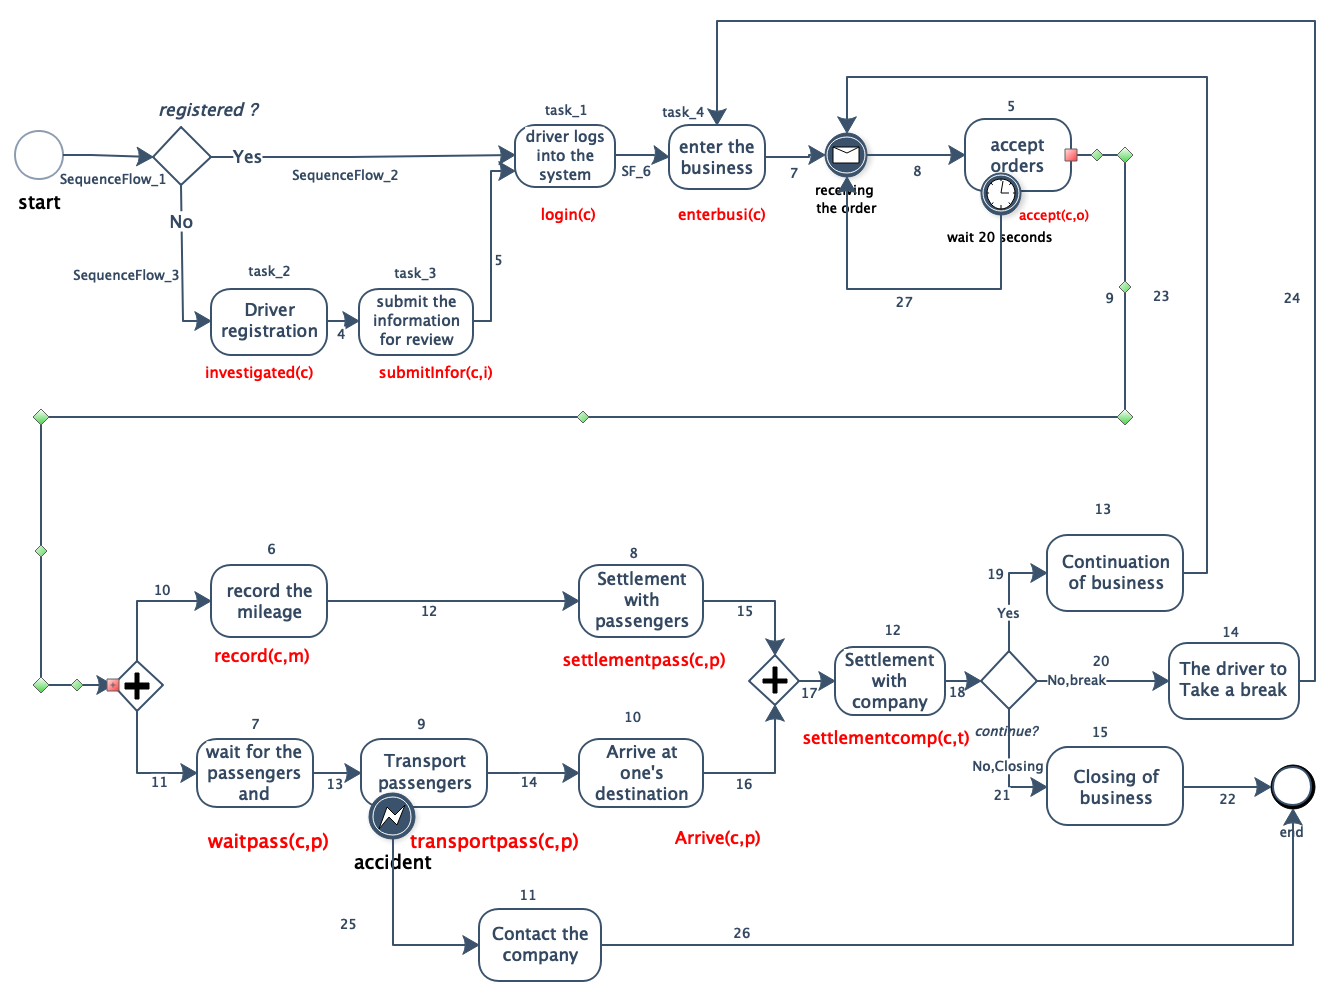
\includegraphics[scale=0.5]{driver_bpmn_128.png}}
\centerline{picture 1. driver bpmn}




\section{bpmn xml code}
\begin{lstlisting}[language={xml}]	%代码段语句

<bpmn:process id="Process_1"> isExecutable="true">
	<bpmn:startEvent id="startEvent_1">
		<bpmn:outgoing>SequenceFlow_1</bpmn:outgoing>
		<bpmn:conditionalStartDefinition />
	</bpmn:startEvent>

	<bpmn:SequenceFlow id="SequenceFlow_1" sourceRef="StartEvet_1" targetRef="exclusiveGateway_1">

	<bpmn:exclusiveGateway id="exclusiveGateway_1" name="regisitered?">
		<bpmn:incoming>SequenceFlow_1</bpmn:incoming>
		<bpmn:outgoing>SequenceFlow_2</bpmn:outgoing>
		<bpmn:outgoing>SequenceFlow_3</bpmn:outgoing>
	</bpmn:exclusiveGateway>

	<bpmn:SequenceFlow id="SequenceFlow_2" sourceRef="exclusiveGateway_1" targetRef="Task_1">
	<bpmn:SequenceFlow id="SequenceFlow_3" sourceRef="exclusiveGateway_1" targetRef="Task_2">


	...
	...

	...


	
	<bpmn:task id="Task_14" name="The driver to Take a break">
		<bpmn:incoming>SequenceFlow_20</bpmn:incoming>
		<bpmn:outgoing>SequenceFlow_24</bpmn:outgoing>
	</bpmn:task> 
	<bpmn:task id="Task_15" name="Closing of business">
		<bpmn:incoming>SequenceFlow_21</bpmn:incoming>
		<bpmn:outgoing>SequenceFlow_22</bpmn:outgoing>
	</bpmn:task> 

	<bpmn:SequenceFlow id="SequenceFlow_23" sourceRef="Task_13" targetRef="IntermediateCatchEvent_1" /> 
	<bpmn:SequenceFlow id="SequenceFlow_24" sourceRef="Task_14" targetRef="Task_4" /> 
	<bpmn:SequenceFlow id="SequenceFlow_22" sourceRef="Task_15" targetRef="endEvent_1" /> 
</bpmn:process>
	\end{lstlisting}






\section{bpmn effect scenarios:}
t13: Scenario(1): $\langle$  $\langle$  t1,t4,t5,\{ $\langle$t6,t8$\rangle$,$\langle$t7,t9,t10$\rangle$ \},t12,t13 $\rangle$, \{  $\langle$t2, t3,$\rangle$   \}  $\rangle$

\noindent t13: Secnario(2): $\langle$  $\langle$  t2,t3,t1,\{$\langle$t6,t8$\rangle$,$\langle$t7,t9,t10$\rangle$ \}$\rangle$,t12,t13$\rangle$	$\rangle$

\noindent t14: Secnario(1): $\langle$  $\langle$  t1,t4,t5,\{$\langle$t6,t8$\rangle$,$\langle$t7,t9,t10$\rangle$ \}$\rangle$,t12,t14$\rangle$, \{  $\langle$t2, t3,$\rangle$   \}  $\rangle$

\noindent t14: Secnario(2): $\langle$  $\langle$  t2,t3,t1,\{$\langle$t6,t8$\rangle$,$\langle$t7,t9,t10$\rangle$ \}$\rangle$,t12,t14$\rangle$	$\rangle$

\noindent t15: Secnario(1): $\langle$  $\langle$  t1,t4,t5,\{$\langle$t6,t8$\rangle$,$\langle$t7,t9,t10$\rangle$ \} $\rangle$,t12,t15$\rangle$, \{  $\langle$t2, t3,$\rangle$   \}	$\rangle$

\noindent t15: Secnario(2): $\langle$  $\langle$  t2,t3,t1,\{$\langle$t6,t8$\rangle$,$\langle$t7,t9,t10$\rangle$ \} $\rangle$,t12,t15$\rangle$	$\rangle$





\section{bpmn cumulative effects:}

enter business: (login(c)\ $\bigvee$ investigated(c) $\bigwedge$\ submitInfor(c,i) ) $\bigwedge$enterbusi(c)

\noindent accept order: (login(c)\ $\bigvee$ investigated(c) $\bigwedge$\ submitInfor(c,i) ) $\bigwedge$enterbusi(c) $\bigwedge$\  accept(c,o)

\noindent settlement with company: (login(c)\ $\bigvee$ investigated(c) $\bigwedge$\ submitInfor(c,i) ) $\bigwedge$enterbusi(c) $\bigwedge$\  accept(c,o) $\bigwedge$\ \ ((record(c,m)$\bigwedge$\ settlementpass(c,p))\ $\bigvee$(waitpass(c,p))\ $\bigwedge$transportpass(c,p)$\bigwedge$Arrive(c,p)) $\bigwedge$settlementcomp(c,t)




\section{cmmn}
\noindent Subprocess of driver bpmn: wait for the passengers:
First, the driver needs to confirm passengers’ position, there is a cmmn stage to describe the process. It is necessary to connect with passengers by phone to get information about the position, then the driver drives to the position. It is a cmmn milestone when meeting the passenger, the next task is confirming the passengers get on the car.
\centerline{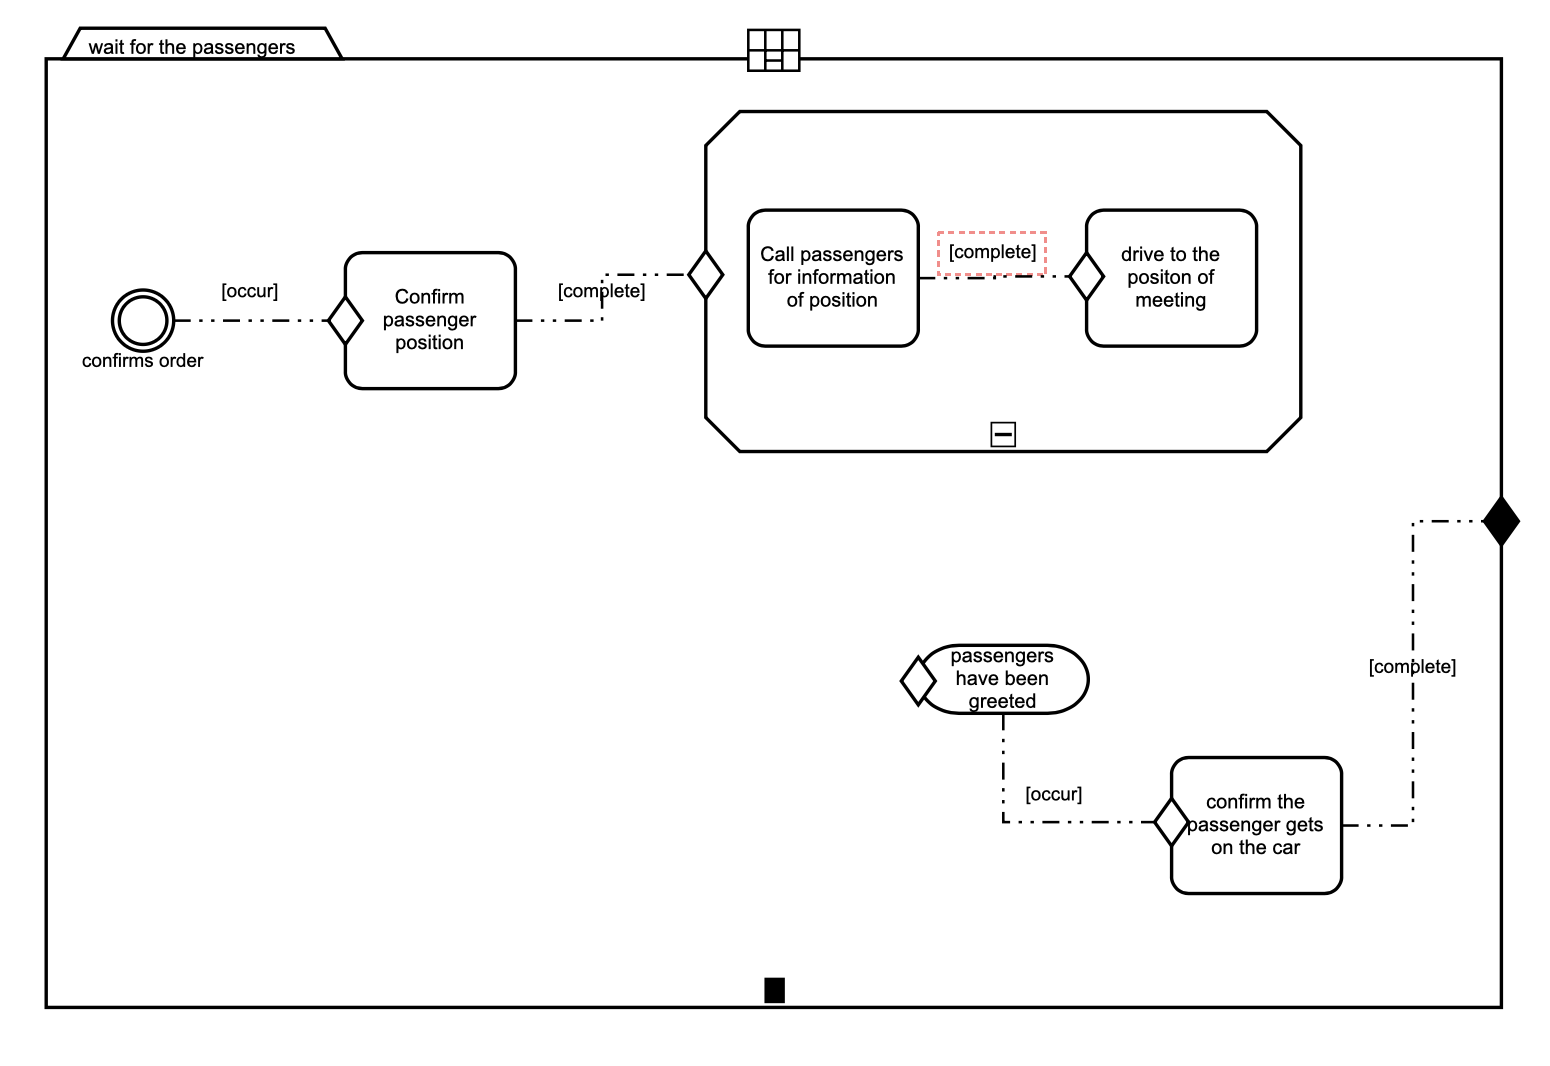
\includegraphics[scale=0.5]{driver_cmmn_128.png}}
\centerline{picture 2. driver cmmn}


\section{rule}
r:Driver receive an order $\vdash$ OBLconform the order$\otimes$ OBLwait for the next order\\
v:Diver conform an order $\vdash$ OBLpick up the passengers

\begin{lstlisting}[language={xml}]	%代码段语句

<Imp label='r'>
	<body>
		Driver receive an order
	</body>
	<head>
		<Behaviour>
			<Obligation>confirm the order</Obligation>
			<Obligation>wait for next order</Obligation>
		</Behaviour>
	</head>
</Imp>
<Imp label 'v'>
	<body>
		confirm the order
	</body>
	<head>
		<Behaviour>
			<Obligation>pick up the passengers</Obligation>
		</Behaviour>
	</head>
</Imp>




\end{lstlisting}


\section{dmn discribe}
This dmn describes the situation of the driver accepting the order. If the order distance is greater than 2 km, the driver would refuse. If the order shows bad passenger credit, the driver would refuse. If the order shows more than 5 passengers, the driver would refuse. If the order is greater than 50km, the driver would refuse.If the order is greater than 50km, but the driver received a surcharge,the driver would accept.If the order shows good passenger credit, the driver would accept.\\

\centerline{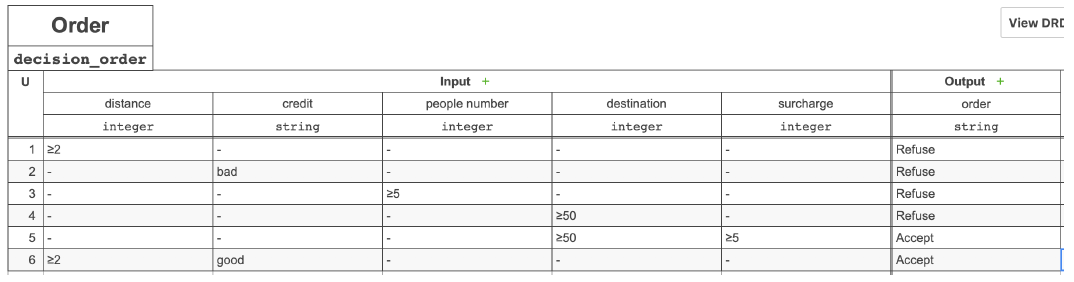
\includegraphics[scale=0.8]{driver_dmn_127.png}}


\section{Petri Net}
This Petri Net describes the process of picking up the passenger and record the mileage until the settlement.\\

\centerline{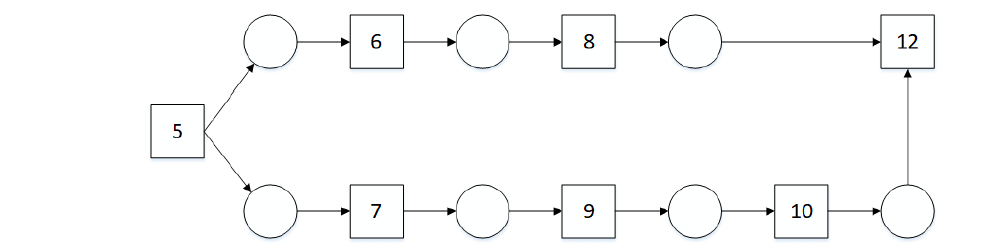
\includegraphics[scale=0.9]{driver_PN_127.png}}
\end{document}
































